\chapter{Execuções para a variação de $E_L$ em torno de $E_0$}

\begin{figure}[htbp]
	\centering
  \begin{tabular}{@{}cc@{}}
    
		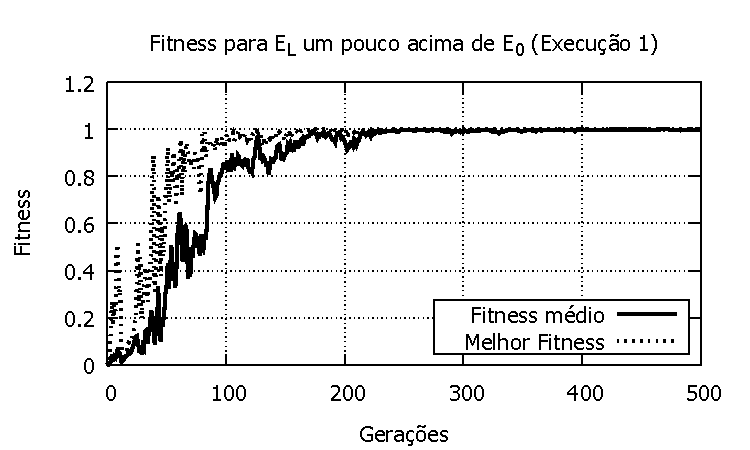
\includegraphics[width=.49\textwidth]{figs/resultados/variandoEL/T1E1_fitness.pdf} &
    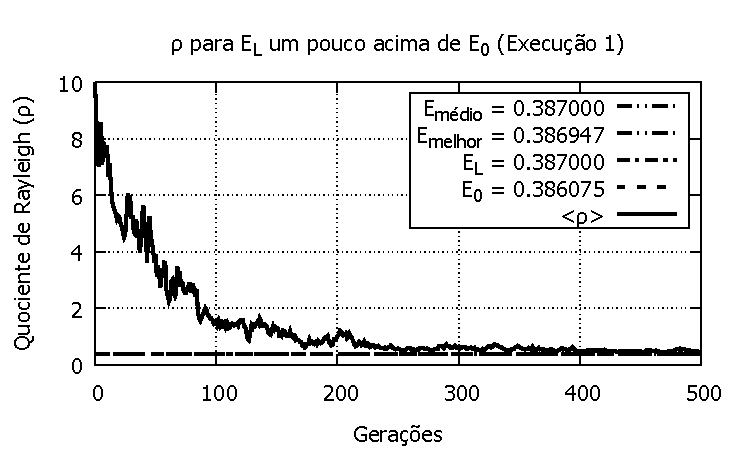
\includegraphics[width=.49\textwidth]{figs/resultados/variandoEL/T1E1_rho.pdf}   \\
		
		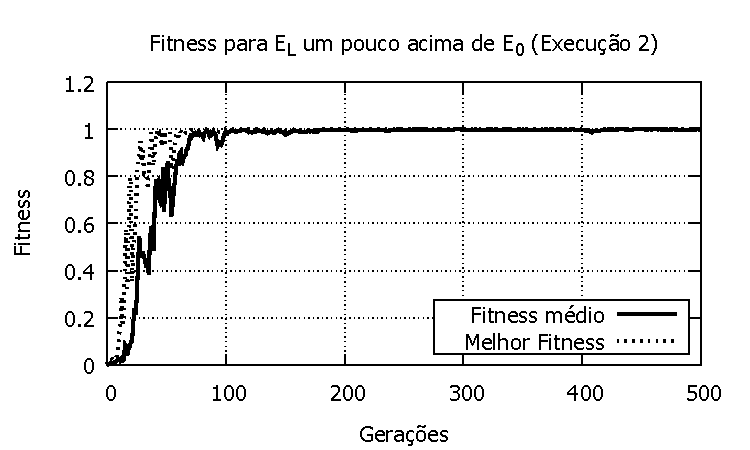
\includegraphics[width=.49\textwidth]{figs/resultados/variandoEL/T1E2_fitness.pdf} &
    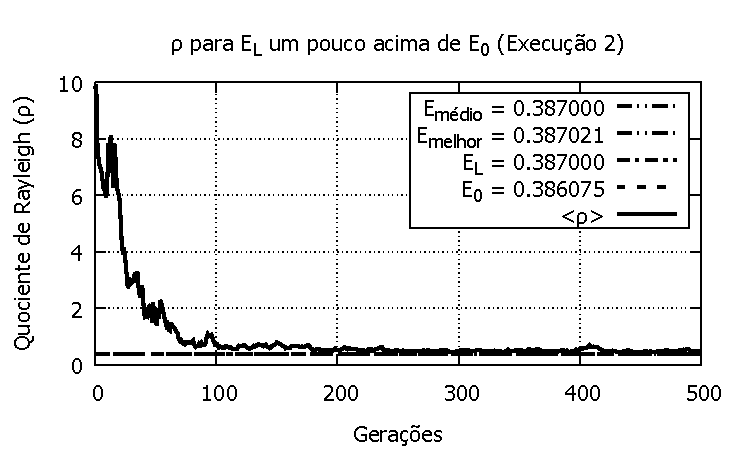
\includegraphics[width=.49\textwidth]{figs/resultados/variandoEL/T1E2_rho.pdf}   \\
		
		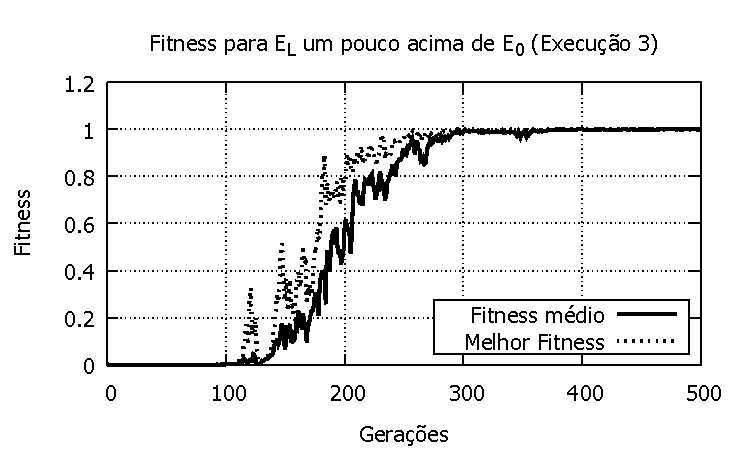
\includegraphics[width=.49\textwidth]{figs/resultados/variandoEL/T1E3_fitness.pdf} &
    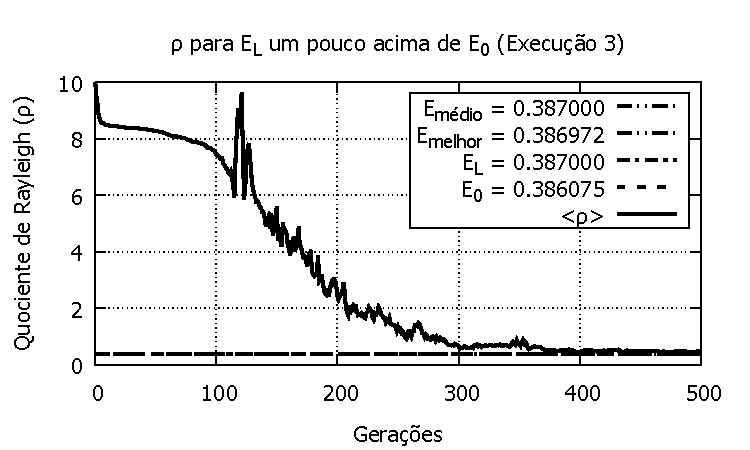
\includegraphics[width=.49\textwidth]{figs/resultados/variandoEL/T1E3_rho.pdf}   \\
		
		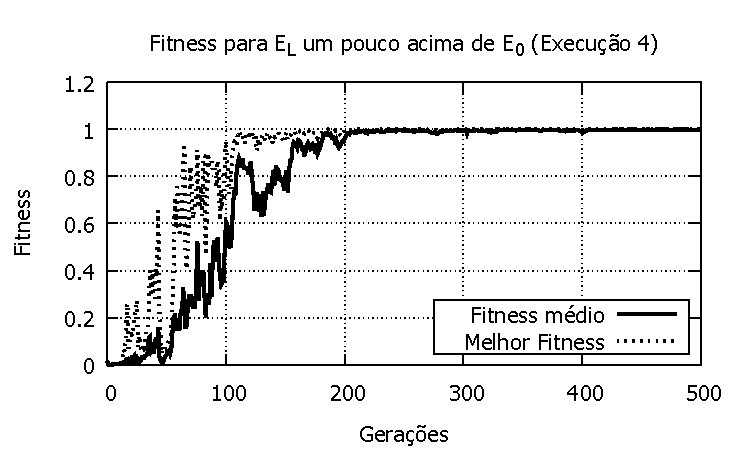
\includegraphics[width=.49\textwidth]{figs/resultados/variandoEL/T1E4_fitness.pdf} &
    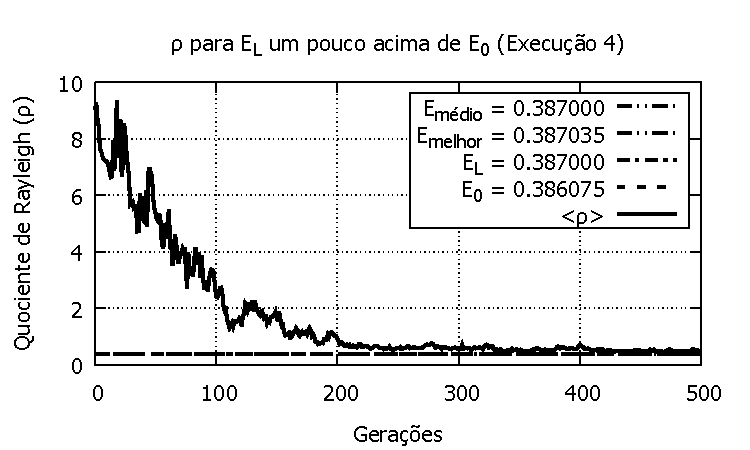
\includegraphics[width=.49\textwidth]{figs/resultados/variandoEL/T1E4_rho.pdf}   \\
		
		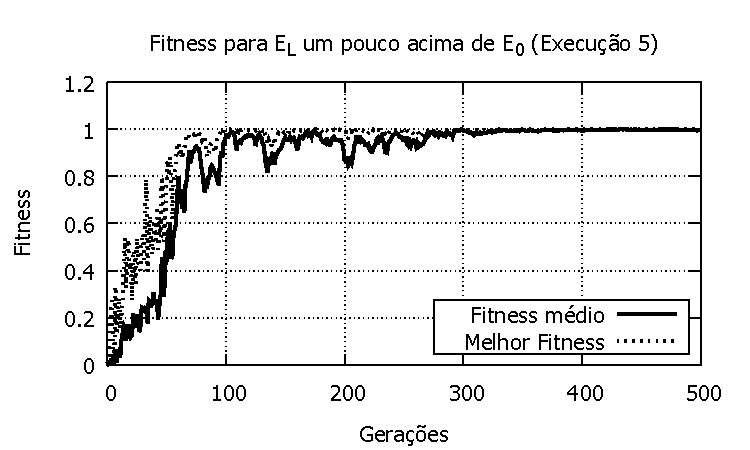
\includegraphics[width=.49\textwidth]{figs/resultados/variandoEL/T1E5_fitness.pdf} &
    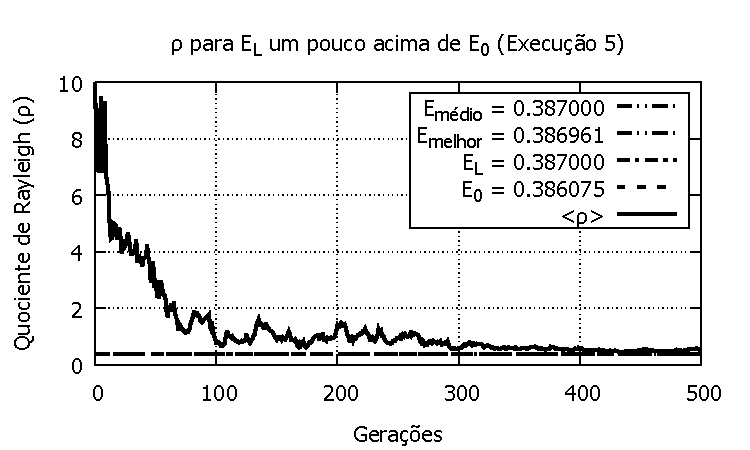
\includegraphics[width=.49\textwidth]{figs/resultados/variandoEL/T1E5_rho.pdf}
		
		%\includegraphics[width=.49\textwidth]{figs/resultados/variandoEL/.pdf} &
    %\includegraphics[width=.49\textwidth]{figs/resultados/variandoEL/.pdf}   \\
		
  \end{tabular}
  \caption{Execuções com o $E_L$ um pouco acima de $E_0$ no \textit{fitness} $f_i = e^{-\lambda(\rho_i - E_L)^2}$. Semente 1445738835, N = 10.}
	\label{fig:variando_EL_pouco_acima}
	\end{figure}
	
%---------------------------------------------------------------------------------------	

	\begin{figure}[htbp]
	\centering
  \begin{tabular}{@{}cc@{}}
    
			
		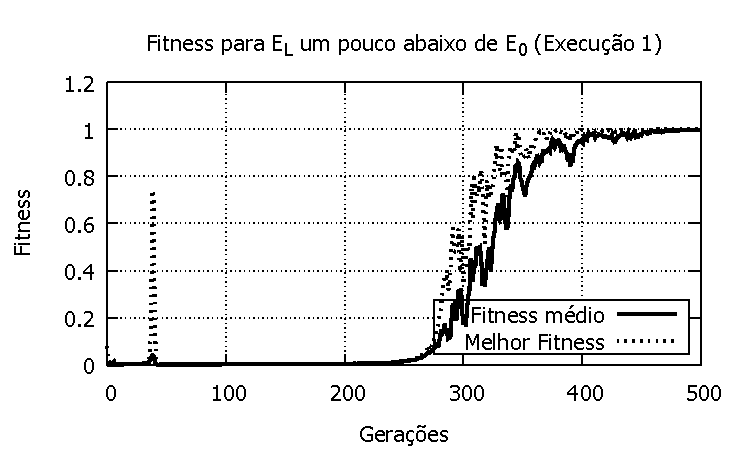
\includegraphics[width=.49\textwidth]{figs/resultados/variandoEL/T2E1_fitness.pdf} &
    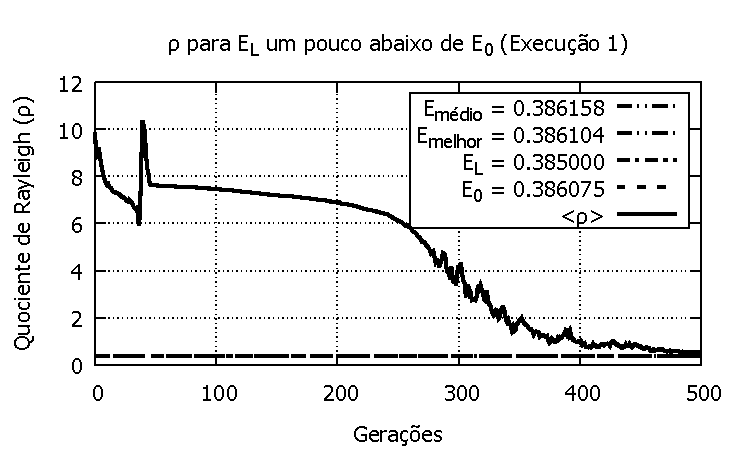
\includegraphics[width=.49\textwidth]{figs/resultados/variandoEL/T2E1_rho.pdf}   \\

		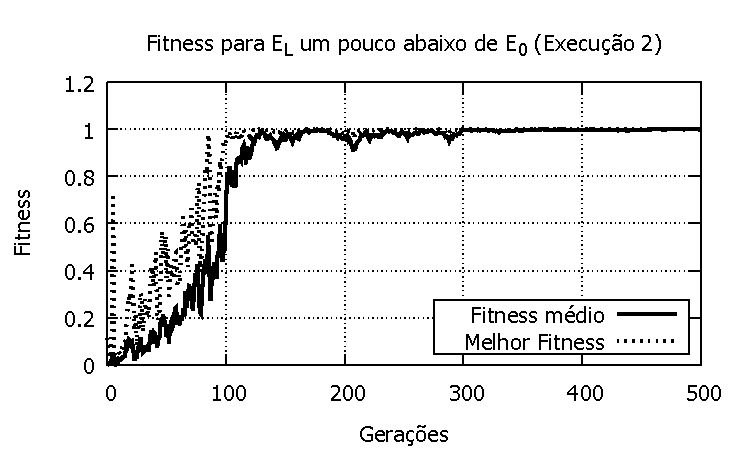
\includegraphics[width=.49\textwidth]{figs/resultados/variandoEL/T2E2_fitness.pdf} &
    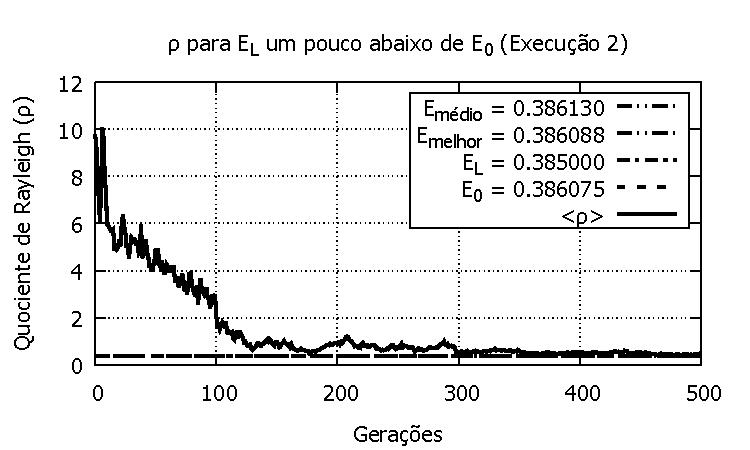
\includegraphics[width=.49\textwidth]{figs/resultados/variandoEL/T2E2_rho.pdf}   \\
		
		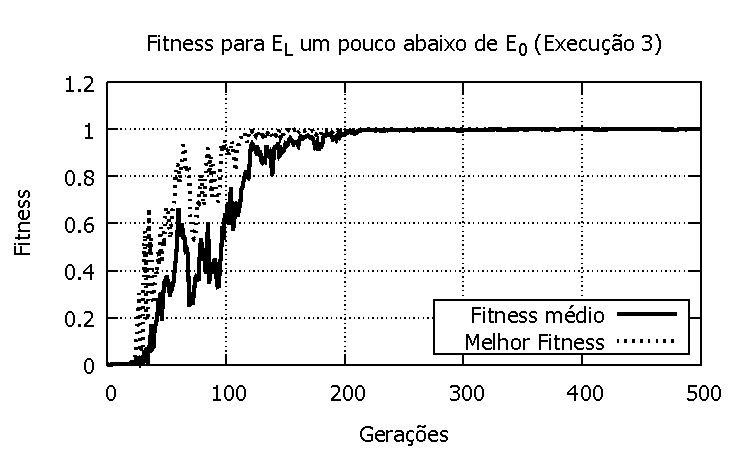
\includegraphics[width=.49\textwidth]{figs/resultados/variandoEL/T2E3_fitness.pdf} &
    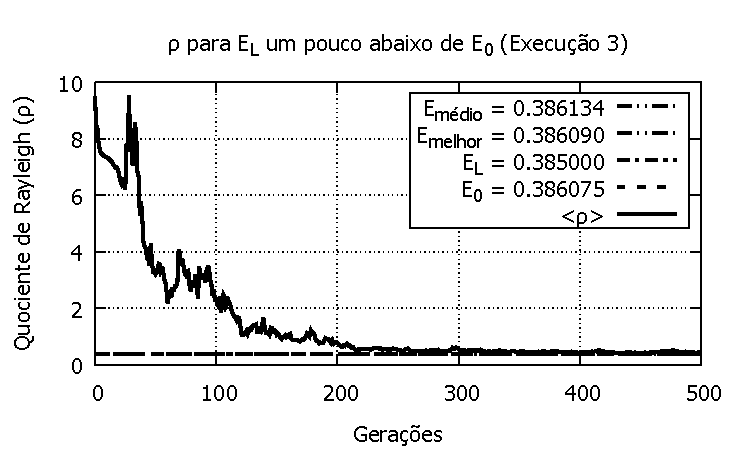
\includegraphics[width=.49\textwidth]{figs/resultados/variandoEL/T2E3_rho.pdf}   \\
		
		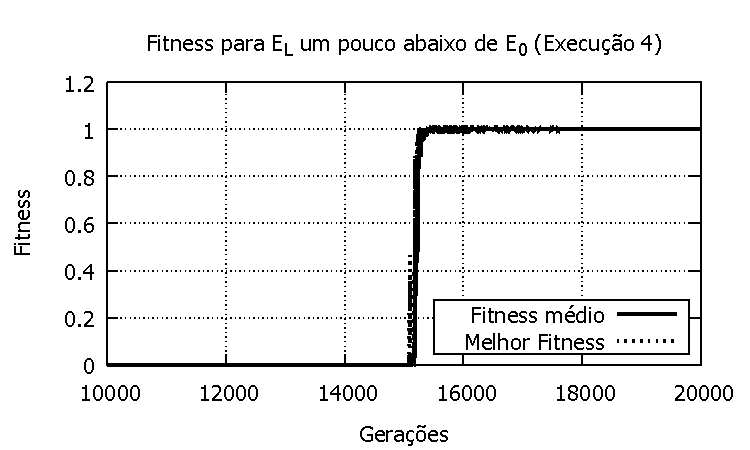
\includegraphics[width=.49\textwidth]{figs/resultados/variandoEL/T2E4_fitness-extendido.pdf} &
    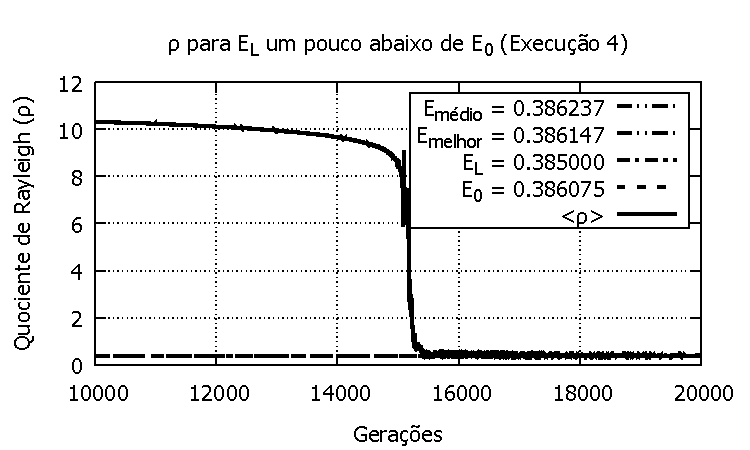
\includegraphics[width=.49\textwidth]{figs/resultados/variandoEL/T2E4_rho_extendido.pdf}   \\
		
		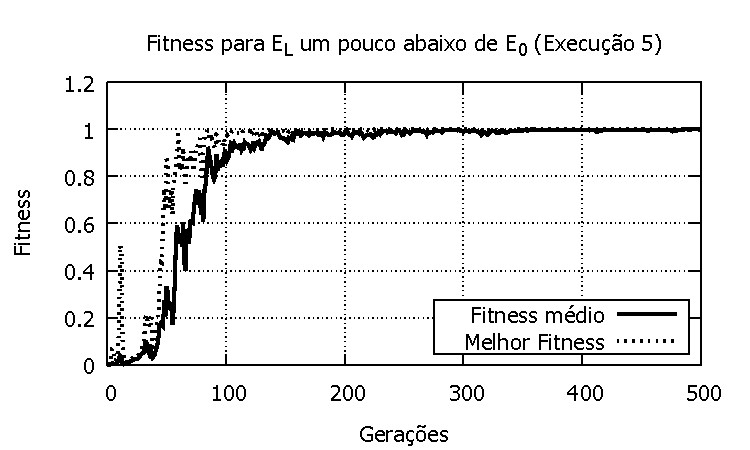
\includegraphics[width=.49\textwidth]{figs/resultados/variandoEL/T2E5_fitness.pdf} &
    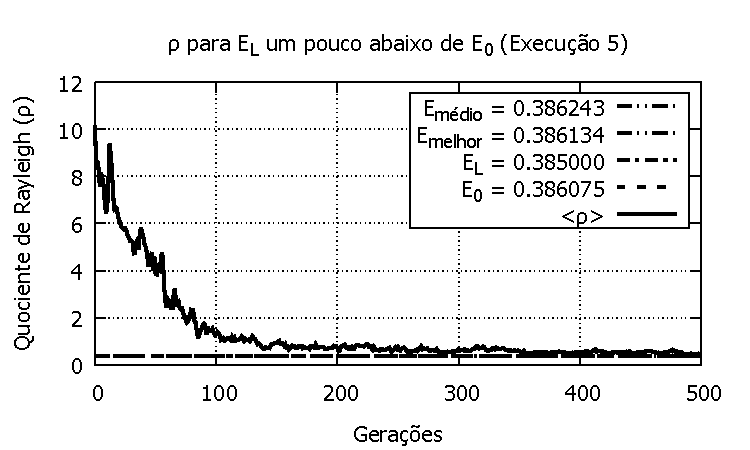
\includegraphics[width=.49\textwidth]{figs/resultados/variandoEL/T2E5_rho.pdf}
		
		%\includegraphics[width=.49\textwidth]{figs/resultados/variandoEL/.pdf} &
    %\includegraphics[width=.49\textwidth]{figs/resultados/variandoEL/.pdf}   \\
		
  \end{tabular}
  \caption{Execuções com o $E_L$ um pouco abaixo de $E_0$ no \textit{fitness} $f_i = e^{-\lambda(\rho_i - E_L)^2}$. Semente 1445738835, N = 10.}
	\label{fig:variando_EL_pouco_abaixo}
	\end{figure}
	
		
%---------------------------------------------------------------------------------------	

	\begin{figure}[htbp]
	\centering
  \begin{tabular}{@{}cc@{}}
    
			
		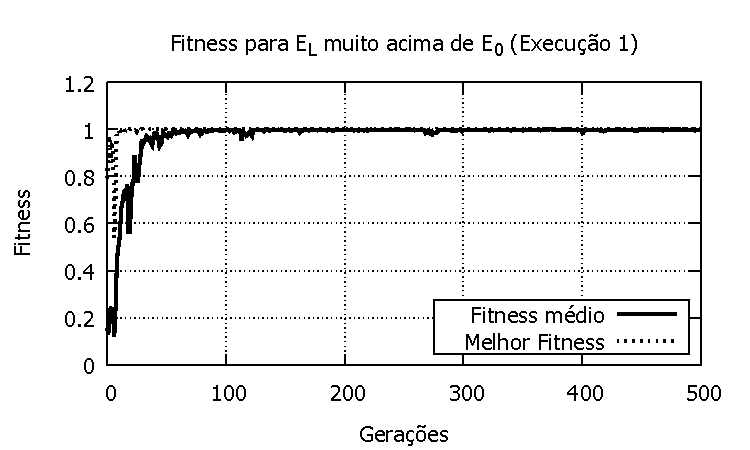
\includegraphics[width=.49\textwidth]{figs/resultados/variandoEL/T3E1_fitness.pdf} &
    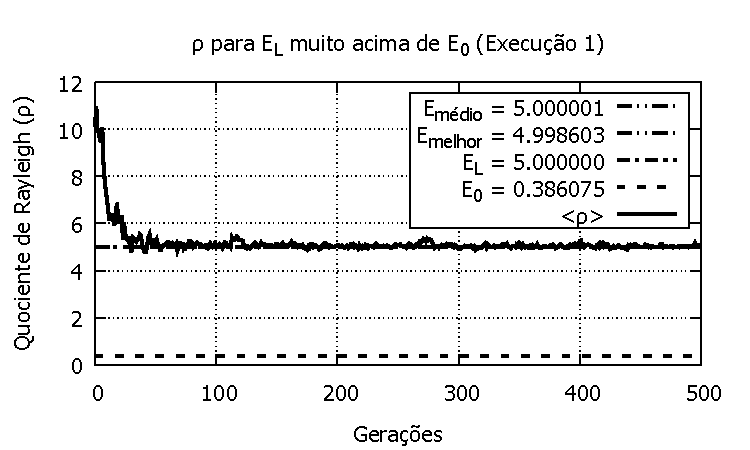
\includegraphics[width=.49\textwidth]{figs/resultados/variandoEL/T3E1_rho.pdf}   \\

		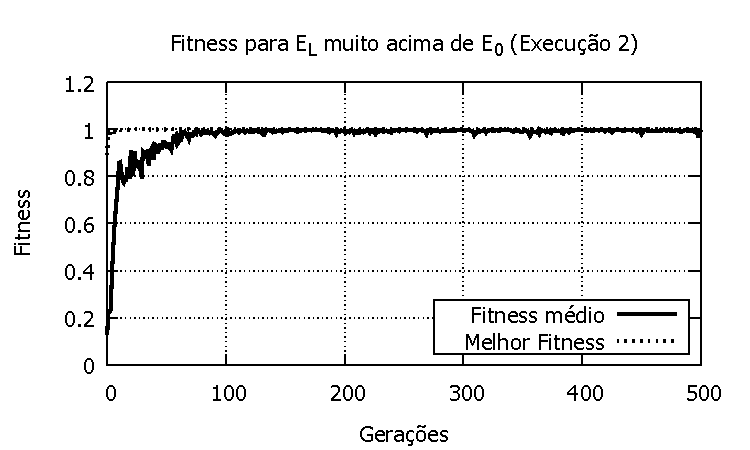
\includegraphics[width=.49\textwidth]{figs/resultados/variandoEL/T3E2_fitness.pdf} &
    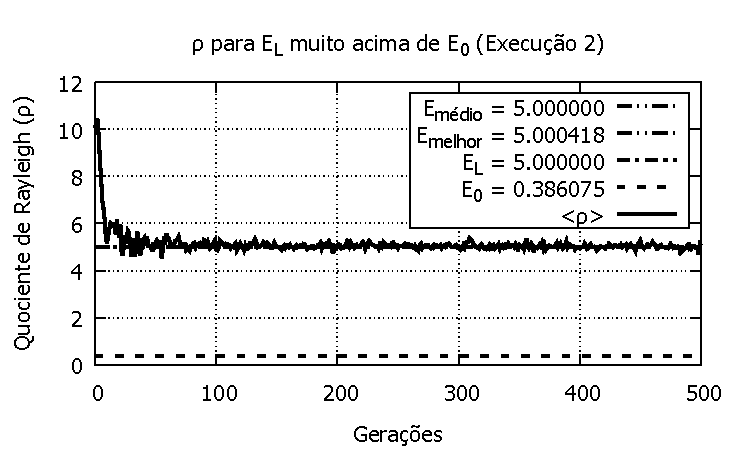
\includegraphics[width=.49\textwidth]{figs/resultados/variandoEL/T3E2_rho.pdf}   \\
		
		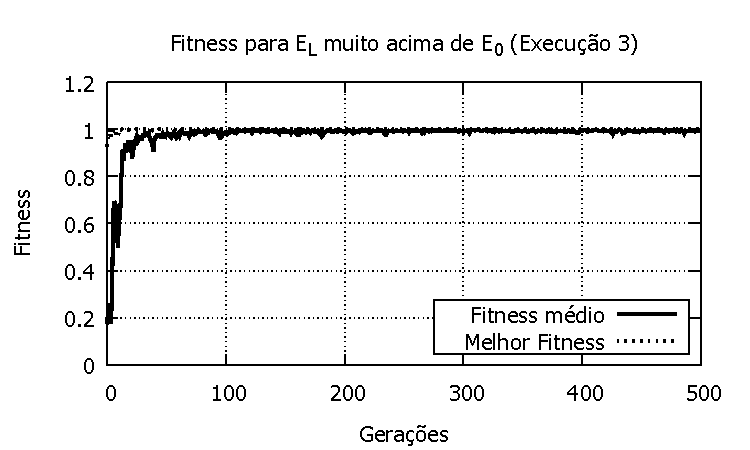
\includegraphics[width=.49\textwidth]{figs/resultados/variandoEL/T3E3_fitness.pdf} &
    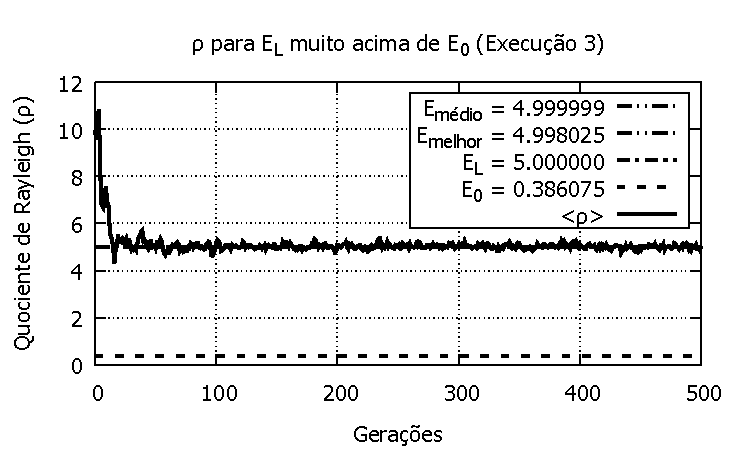
\includegraphics[width=.49\textwidth]{figs/resultados/variandoEL/T3E3_rho.pdf}   \\
		
		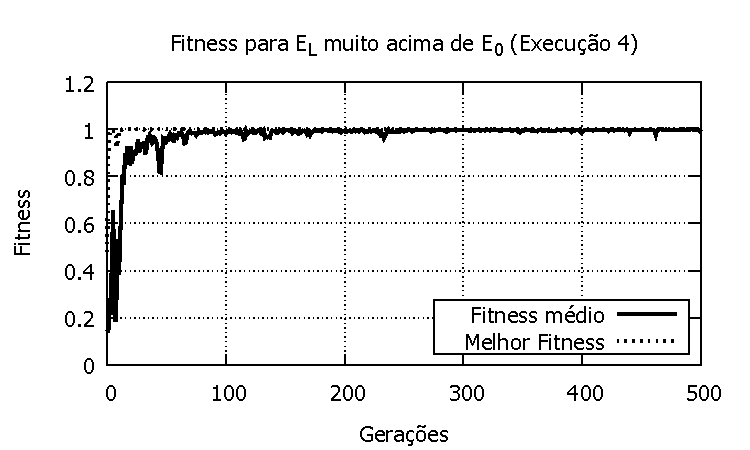
\includegraphics[width=.49\textwidth]{figs/resultados/variandoEL/T3E4_fitness.pdf} &
    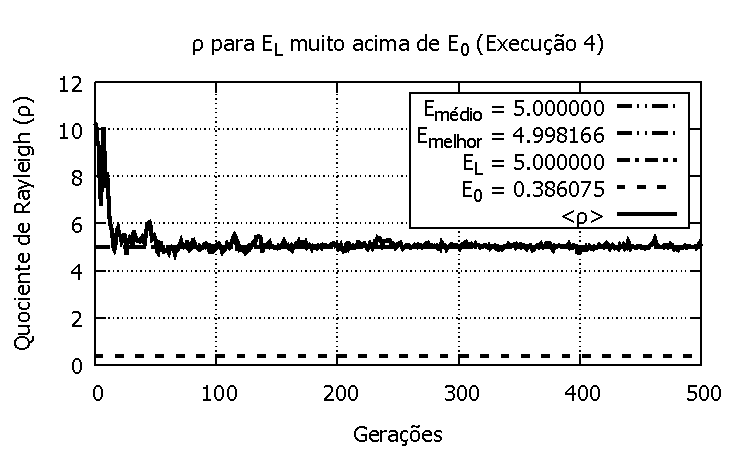
\includegraphics[width=.49\textwidth]{figs/resultados/variandoEL/T3E4_rho.pdf}   \\
		
		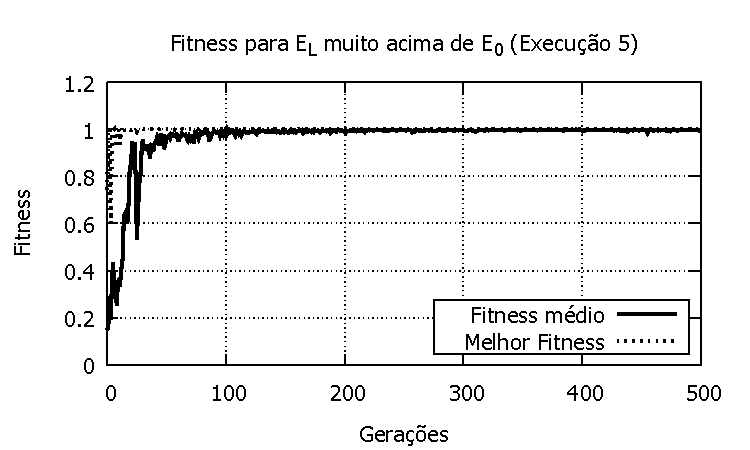
\includegraphics[width=.49\textwidth]{figs/resultados/variandoEL/T3E5_fitness.pdf} &
    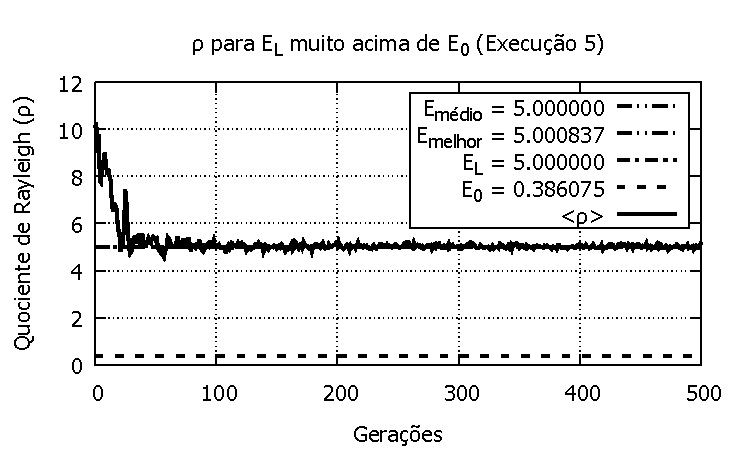
\includegraphics[width=.49\textwidth]{figs/resultados/variandoEL/T3E5_rho.pdf}
		
		%\includegraphics[width=.49\textwidth]{figs/resultados/variandoEL/.pdf} &
    %\includegraphics[width=.49\textwidth]{figs/resultados/variandoEL/.pdf}   \\
		
  \end{tabular}
  \caption{Execuções com o $E_L$ muito acima de $E_0$ no \textit{fitness} $f_i = e^{-\lambda(\rho_i - E_L)^2}$. Semente 1445738835, N = 10.}
	\label{fig:variando_EL_muito_acima}
	\end{figure}
	
%---------------------------------------------------------------------------------------	

	\begin{figure}[htbp]
	\centering
  \begin{tabular}{@{}cc@{}}
    
			
		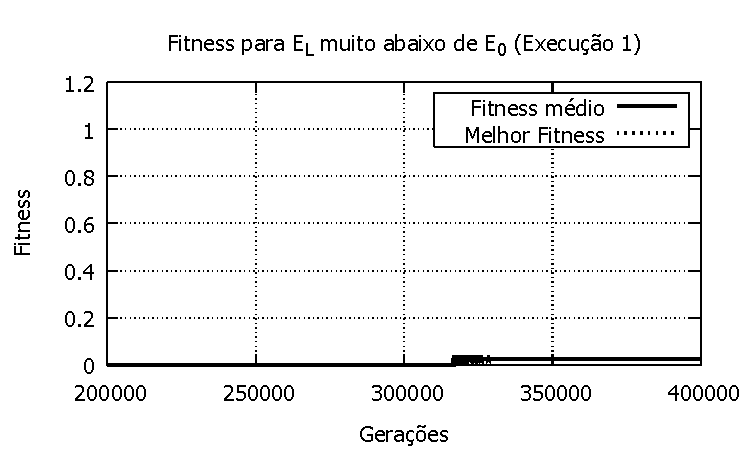
\includegraphics[width=.49\textwidth]{figs/resultados/variandoEL/T4E1_fitness-extendido.pdf} &
    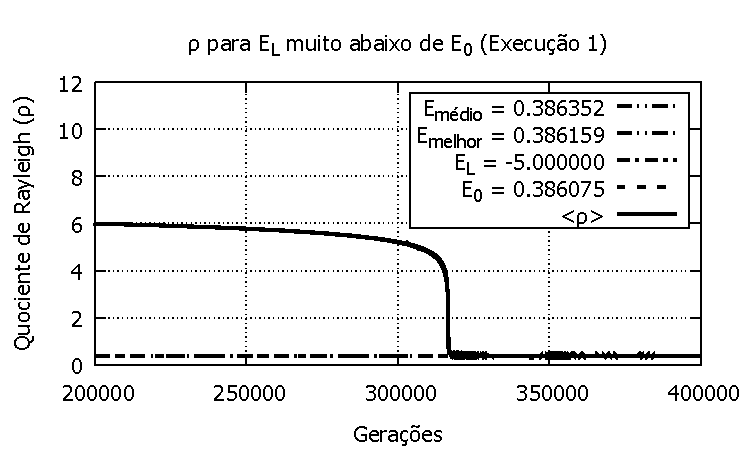
\includegraphics[width=.49\textwidth]{figs/resultados/variandoEL/T4E1_rho_extendido.pdf}   \\

		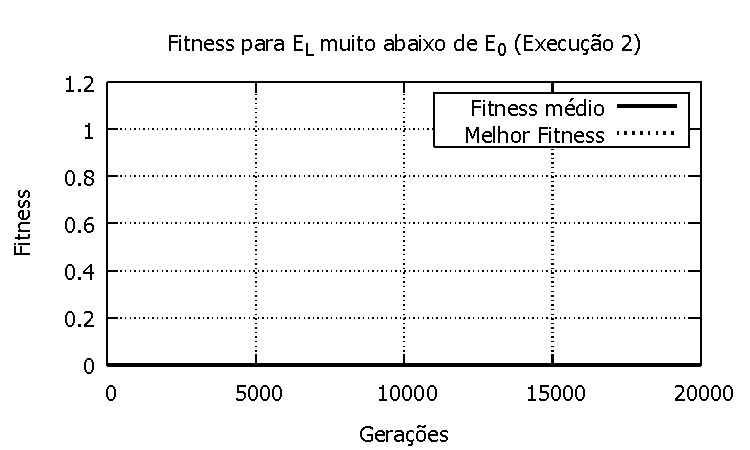
\includegraphics[width=.49\textwidth]{figs/resultados/variandoEL/T4E2_fitness-extendido.pdf} &
    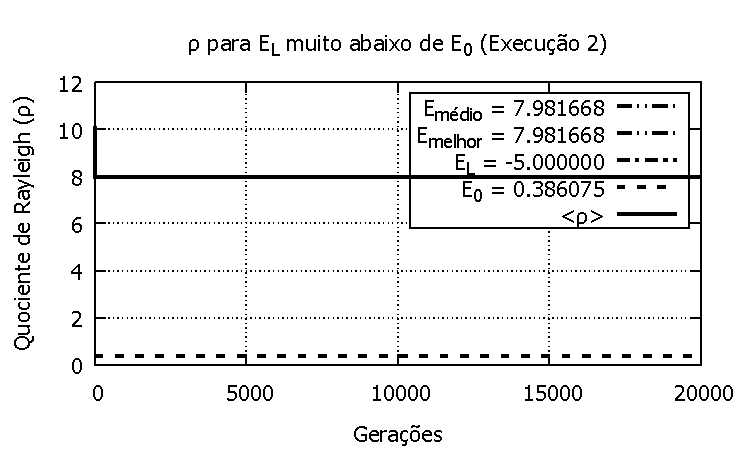
\includegraphics[width=.49\textwidth]{figs/resultados/variandoEL/T4E2_rho_extendido.pdf}   \\
		
		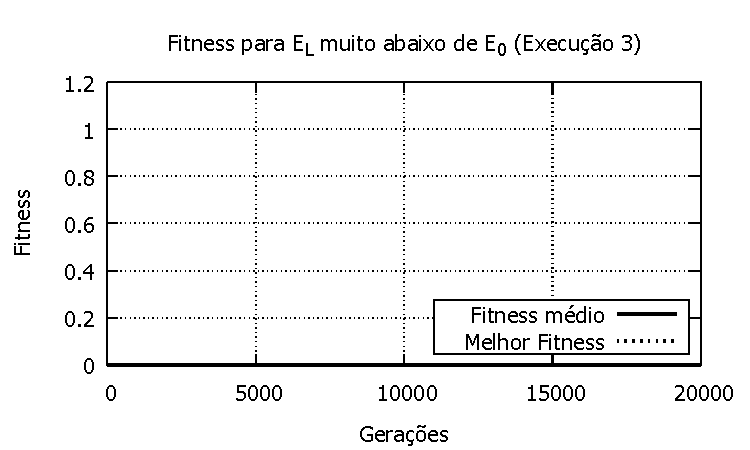
\includegraphics[width=.49\textwidth]{figs/resultados/variandoEL/T4E3_fitness-extendido.pdf} &
    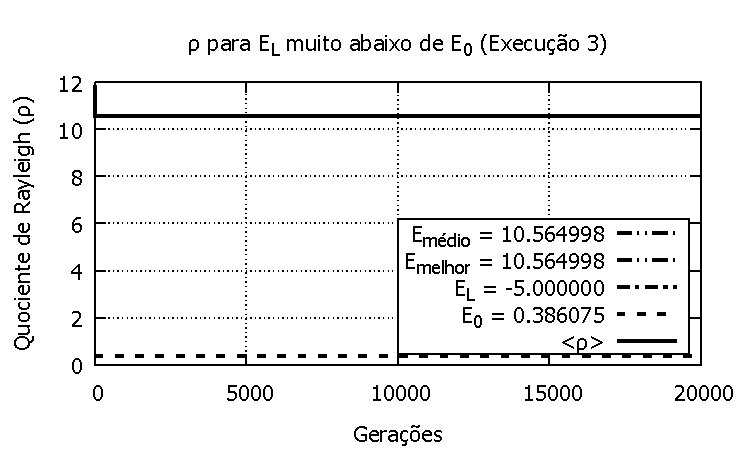
\includegraphics[width=.49\textwidth]{figs/resultados/variandoEL/T4E3_rho_extendido.pdf}   \\
		
		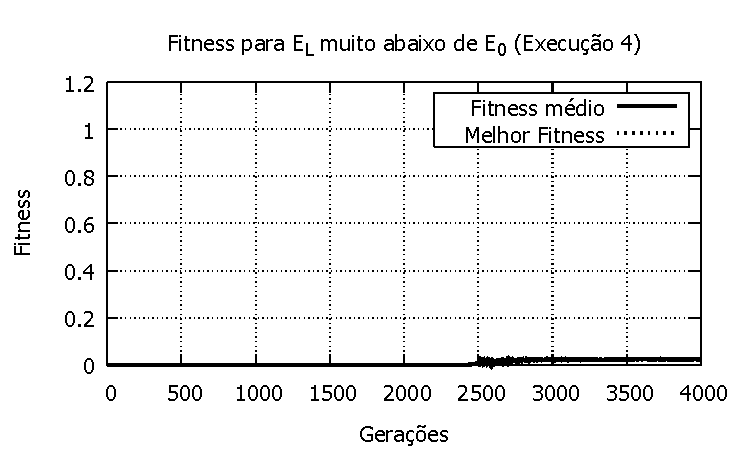
\includegraphics[width=.49\textwidth]{figs/resultados/variandoEL/T4E4_fitness-extendido.pdf} &
    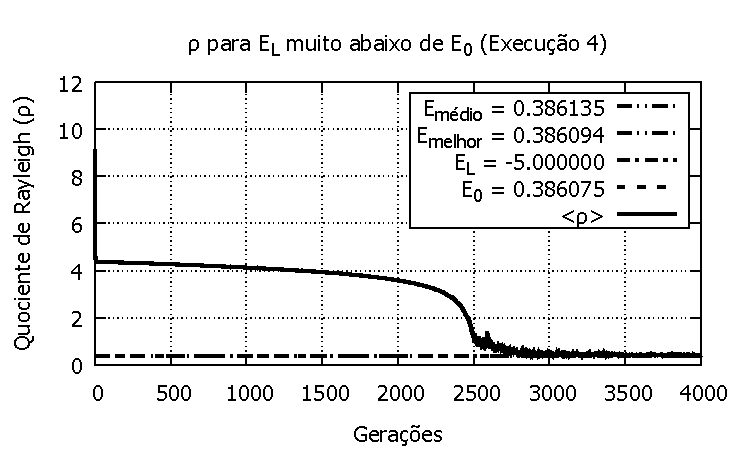
\includegraphics[width=.49\textwidth]{figs/resultados/variandoEL/T4E4_rho_extendido.pdf}   \\
		
		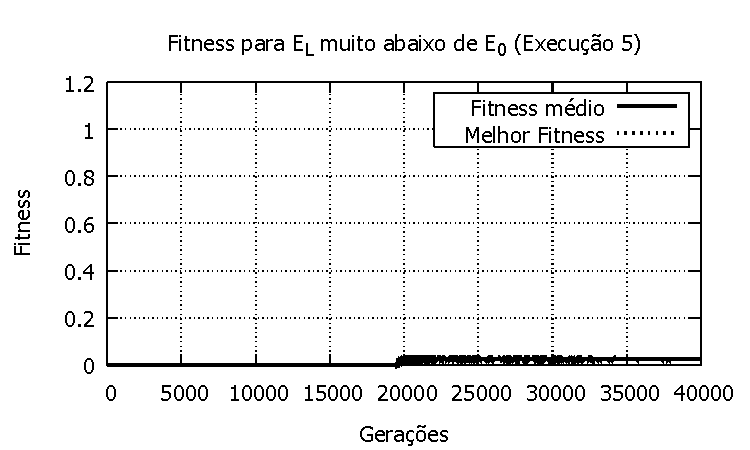
\includegraphics[width=.49\textwidth]{figs/resultados/variandoEL/T4E5_fitness-extendido.pdf} &
    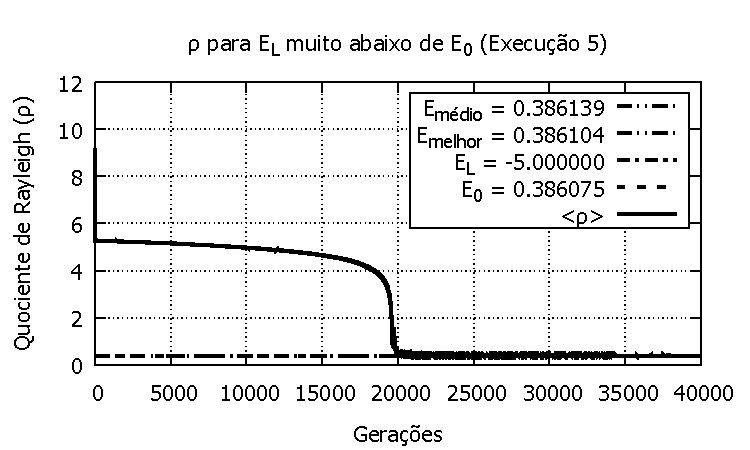
\includegraphics[width=.49\textwidth]{figs/resultados/variandoEL/T4E5_rho_extendido.pdf}
		
		%\includegraphics[width=.49\textwidth]{figs/resultados/variandoEL/.pdf} &
    %\includegraphics[width=.49\textwidth]{figs/resultados/variandoEL/.pdf}   \\
		
  \end{tabular}
  \caption{Execuções com o $E_L$ muito abaixo de $E_0$ no \textit{fitness} $f_i = e^{-\lambda(\rho_i - E_L)^2}$. Semente 1445738835, N = 10.}
	\label{fig:variando_EL_muito_abaixo}
	\end{figure}